\linespread{1.3}
\section{Задание 3. Ряд Тейлора}
\subsection{Задание}
Исследуйте ряд Тейлора функции  в точке. Изобразите графически несколько различных  частичных сумм ряда и график исходной функции. Проведите анализ полученных результатов.\\
\begin{equation*}
	f(x) = ln(\frac{x - 2}{7 - 2x}), \quad x_0 = 3
\end{equation*}
\begin{flalign*} 
	&\text{Найдем первые 5 производных и их значения в точке x_0}&&\\
	&f(3) = ln(1) = 0&&\\
	1) \ &f'(x) = \frac{3}{(x - 2)(7 - 2x)} &&\\
	&f'(3) = 3 &&\\
	2) \ &f''(x) = \frac{12x - 33}{(-2x^2 + 11x - 14)^2} &&\\
	&f''(3) = 3 &&\\
	3) \ &f'''(x) = \frac{72x^2 - 396x + 558}{(-2x^2 + 11x - 14)^3}&&\\
	&f'''(3) = 18 &&\\
	4) \ &f^{IV}(x) = \frac{576x^3 - 4752x^2 + 13392x - 12870}{(-2x^2 + 11x - 14)^4}&&\\
	&f^{IV}(3) = 90 &&\\
	5) \ &f^{V}(x) = \frac{5760x^4 - 63360x^3 + 267840x^2 - 514800x + 378792}{(-2x^2 + 11x - 14)^5}&&\\
	&f^{V}(3) = 792 &&\\
	\text{Подставим значения в ряд: }& &&\\
	&f(x) = y(3) + y'(3)(x - 3) + \frac{y''(3)(x - 3)^2}{2!} + \frac{y'''(3)(x - 3)^3}{3!} + \frac{y^{IV}(3)(x - 3)^4}{4!} + &&\\
	& + \frac{y^{V}(3)(x - 3)^5}{5!} + \dots = &&\\
	&= 0 + 3 \cdot (x - 3) + 3 \cdot \frac{(x - 3)^2}{2!} + 18 \cdot \frac{(x - 3)^3}{3!} + 90 \cdot \frac{(x - 3)^4}{4!}  + 792 \cdot \frac{(x - 3)^5}{5!}  + \dots = &&\\
	&= 0 + 3 \cdot (x - 3) + \frac{1 \cdot 3}{2} \cdot (x - 3)^2 + \frac{3 \cdot 3}{3} \cdot (x - 3)^3 + \frac{5 \cdot 3}{4} \cdot (x - 3)^4 &&\\
	&+ \frac{11 \cdot 3}{5} \cdot (x - 3)^5  + \dots = &&\\
	&= \sum_{n=1}^\infty \frac{2^n + (-1)^{n + 1}}{n}(x - 3)^n&& \\
\end{flalign*}
\begin{flalign*}
	&\text{Найдем область сходимости:}&&\\
	& R = \lim_{n \to \infty} \bigg|\frac{c_n}{c_{n + 1}}\bigg| = \lim_{n \to \infty} \bigg|\frac{(2^n + (-1)^{n + 1})(n + 1)}{n(2^{n + 1} + (-1)^{n + 2})}\bigg| = \frac{1}{2} &&\\
	&\text{Рассмотрим граничные точки:}&&\\
	&\frac{1}{2^n} \cdot \frac{2^n + (-1)^{n + 1}}{n} \geq \frac{1}{2^n} \cdot \frac{2^n - 1}{n}&&\\
	&\text{Сравним ряд с гармоническим:}&&\\
	& \lim_{n \to \infty} \frac{\frac{2^n - 1}{2^n \cdot n}}{\frac{1}{n}} = 1  => \text{ряд расходится}&&\\
	&\frac{1}{(-2)^n} \cdot \frac{2^n + (-1)^{n + 1}}{n}&&\\
	&\text{Рассмотрим первые 3 члена ряда:}&&\\
	&-\frac{3}{2}, \frac{3}{8}, -\frac{3}{8}&&\\
	&\text{Модуль каждого последующего члена ряда не меньше предыдущего, а значит ряд расходится по признаку}&&\\
	&\text{Лейбница}&&\\
	&\text{Таким образом область сходимости исходного ряда: } (2,5; 3,5)&&\\
\end{flalign*}
\begin{center}
	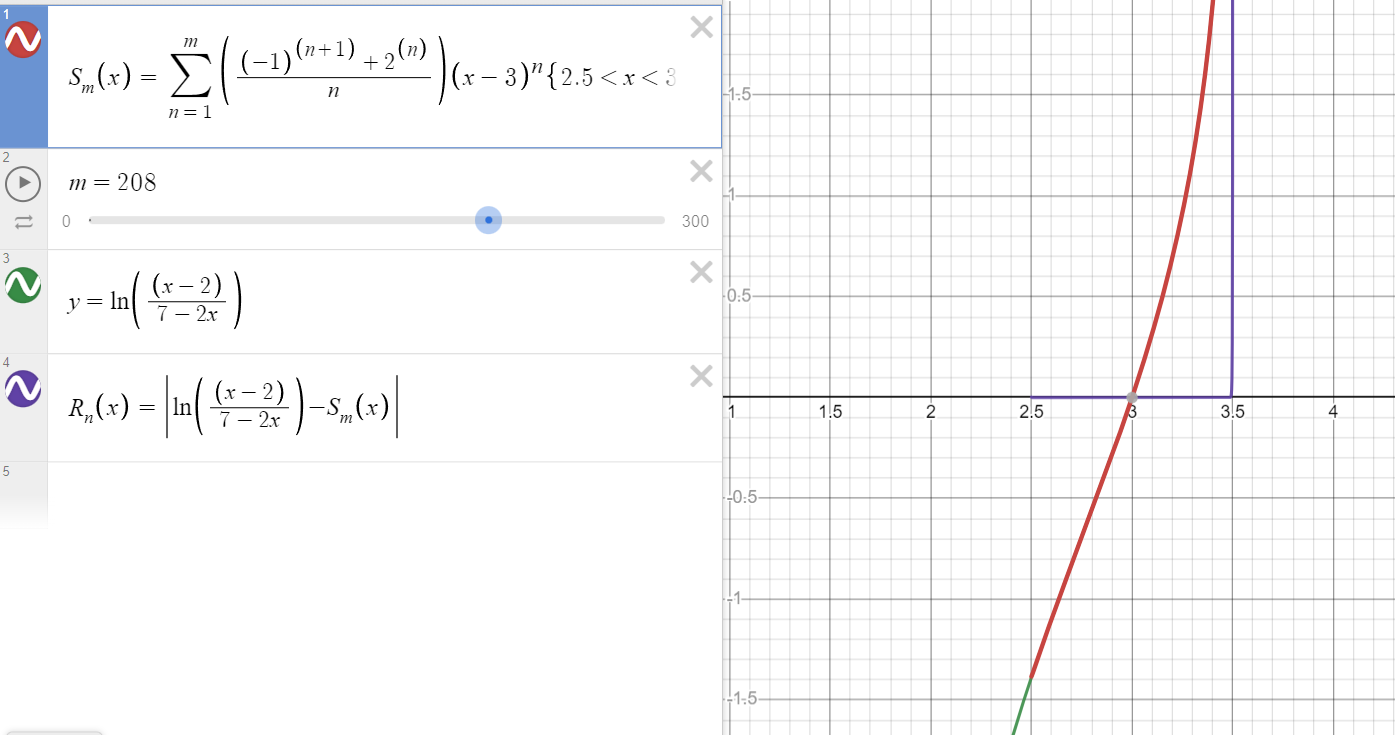
\includegraphics[width=0.9\linewidth]{task2_1_img1}\\
	\url{https://www.desmos.com/calculator/8d2svsbywe?lang=ru}
\end{center}
